\documentclass[noindent, nochapname]{tudexercise}
\usepackage[utf8]{inputenc}
\usepackage[english]{babel}
\usepackage{amsmath}
\usepackage{listings}
\title{Natural Language Processing and the Web}
\subtitle{Machine Learning Project - Documentation}
\subsubtitle{Benedikt Lins (1799381) und Stefan Thaut (1800351)\\
			Department 20 - Computer Science\\
			\today}
\setlength{\parindent}{0em} 
\begin{document}
	\lstset{language=Java}
	\maketitle
	
	\section{Foundations}
		In this Machine Learning Project we want to develop a named entity recognizer based on a machine learning approach. A named entity is a set of tokens, which form a name. Examples are "New York" or "Angela Merkel". We use a Conditional Random Field as the machine learning model.\\
		Our training set contains a set of tokens with a chunk-annotation and the associated named entity class relating to the IOB-notation. We also have a german training set, that additionally contains a lemma for the given token.\\
		An analysis for the english training set shows, that about 83 \% of all tokens are no named entities, as we can see in figure \ref{fig:class_distribution}
		
		\begin{figure}[h]
			\centering
			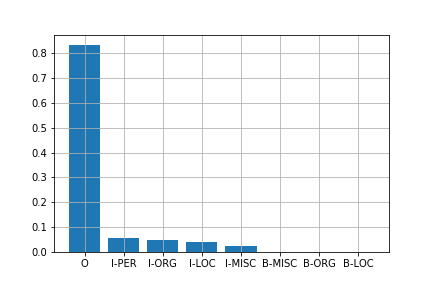
\includegraphics[scale=0.6]{img/class_distribution.png}
			\caption{Class distribution of the english training set}
			\label{fig:class_distribution}
		\end{figure}
	
	\section{Additional features}
		\subsection{Last two characters of a token}
			At first we have tried to use the last two characters (ltc) of a token as a feature. For the meaningfulness of this feature, we analysed the most frequent ltc for the class \textit{O} and for the tokens, that are not in the class \textit{O}. The ten most frequent ltc are presented in figure \ref{fig:ten_most_frequent_ltc}.
			
			\begin{figure}[h]
				\centering
				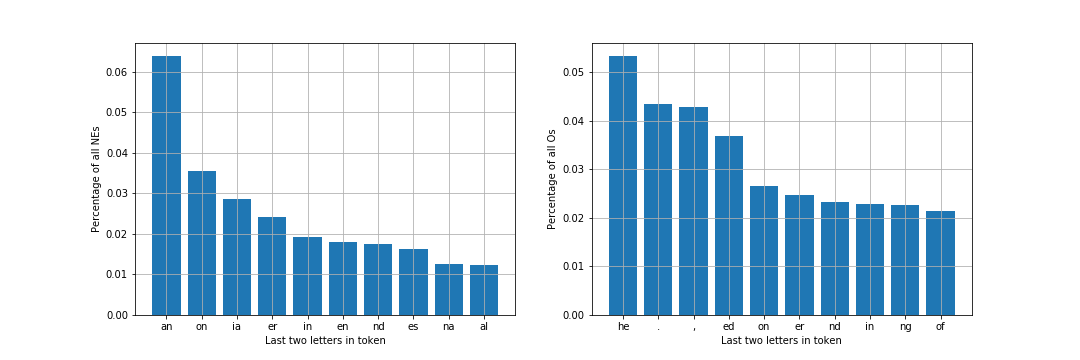
\includegraphics[scale=0.5]{img/last_two_letters_per_class.png}
				\caption{This figures show the ten most frequent ltc. The right side shows the ltc for the class \textit{O} and the left side shows the ltc for all tokens, that are not in class \textit{O}}
				\label{fig:ten_most_frequent_ltc}
			\end{figure}
			
			As we can see, about six percent of all named entities end with "an" and about five percent of all non named entities end with "he". In the next step it is important to find out, if some endings are typical for named entities or for non named entities. So we examined the appearances of the most frequent ltc of named entities in tokens that are non named entities and vice versa. The results for the ten most frequent ltc are shown in figure \ref{fig:ten_most_frequent_comparison}. The left side shows the comparison for the most frequent ltc of named entities. The blue curve represents the occurences of the ltc in named entities and the orange curve represents the occurences of the ltc in non named entities. So we can imply, that the greater the distance between the both curves is, the more specific the ltc is for the class. We identified the ltc "an", "ia", and "na" as typical for named entities and analogously the ltc "he", ".", ",", "ed" and "of" as typical for non named entities.
			
			\begin{figure}[h]
				\centering
				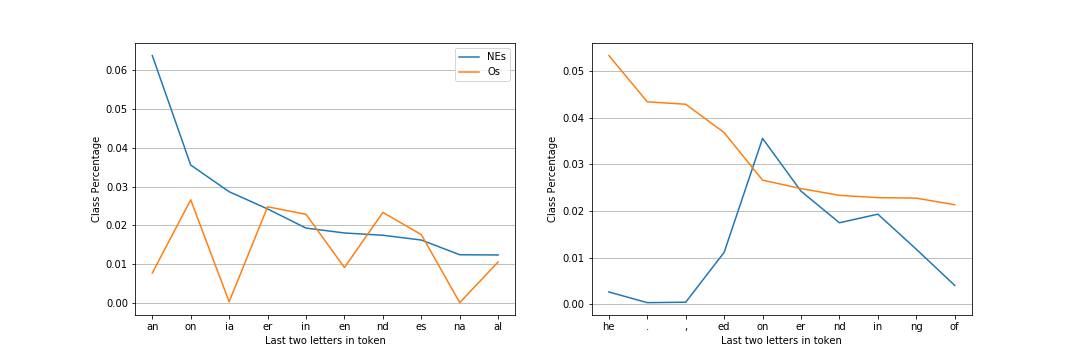
\includegraphics[scale=0.5]{img/last_two_letters_comparison.png}
				\caption{This figures show the percentages of the ten most frequent ltc in comparison of the classes named entity and non named entity}
				\label{fig:ten_most_frequent_ltc}
			\end{figure}

\end{document}